%%%%%%%%%%%%%%%%%%%%%%%%%%%%%%%%%%%%%%%%%
% Beamer Presentation
% LaTeX Template
% Version 1.0 (10/11/12)
%
% This template has been downloaded from:
% http://www.LaTeXTemplates.com
%
% License:
% CC BY-NC-SA 3.0 (http://creativecommons.org/licenses/by-nc-sa/3.0/)
%
%%%%%%%%%%%%%%%%%%%%%%%%%%%%%%%%%%%%%%%%%

%----------------------------------------------------------------------------------------
%	PACKAGES AND THEMES
%----------------------------------------------------------------------------------------

\documentclass{beamer}

\mode<presentation> {

% The Beamer class comes with a number of default slide themes
% which change the colors and layouts of slides. Below this is a list
% of all the themes, uncomment each in turn to see what they look like.

%\usetheme{default}
%\usetheme{AnnArbor}
%\usetheme{Antibes}
%\usetheme{Bergen}
%\usetheme{Berkeley}
%\usetheme{Berlin}
%\usetheme{Boadilla}
%\usetheme{CambridgeUS}
%\usetheme{Copenhagen}
%\usetheme{Darmstadt}
%\usetheme{Dresden}
%\usetheme{Frankfurt}
%\usetheme{Goettingen}
%\usetheme{Hannover}
%\usetheme{Ilmenau}
%\usetheme{JuanLesPins}
%\usetheme{Luebeck}
\usetheme{Madrid}
\usepackage{subcaption}
\usepackage{kantlipsum}
\usepackage{xcolor}


\usepackage{calligra}
\DeclareMathAlphabet{\mathcalligra}{T1}{calligra}{m}{n}
\DeclareFontShape{T1}{calligra}{m}{n}{<->s*[2.2]callig15}{}
\newcommand{\scripty}[1]{\ensuremath{\mathcalligra{#1}}}

%\usetheme{Malmoe}
%\usetheme{Marburg}
%\usetheme{Montpellier}
%\usetheme{PaloAlto}
%\usetheme{Pittsburgh}
%\usetheme{Rochester}
%\usetheme{Singapore}
%\usetheme{Szeged}
%\usetheme{Warsaw}

% As well as themes, the Beamer class has a number of color themes
% for any slide theme. Uncomment each of these in turn to see how it
% changes the colors of your current slide theme.

%\usecolortheme{albatross}
%\usecolortheme{beaver}
%\usecolortheme{beetle}
%\usecolortheme{crane}
%\usecolortheme{dolphin}
%\usecolortheme{dove}
%\usecolortheme{fly}
%\usecolortheme{lily}
%\usecolortheme{orchid}
%\usecolortheme{rose}
%\usecolortheme{seagull}
%\usecolortheme{seahorse}
%\usecolortheme{whale}
%\usecolortheme{wolverine}

%\setbeamertemplate{footline} % To remove the footer line in all slides uncomment this line
%\setbeamertemplate{footline}[page number] % To replace the footer line in all slides with a simple slide count uncomment this line

%\setbeamertemplate{navigation symbols}{} % To remove the navigation symbols from the bottom of all slides uncomment this line
}

\usepackage{graphicx} % Allows including images
\usepackage{booktabs} % Allows the use of \toprule, \midrule and \bottomrule in tables

%----------------------------------------------------------------------------------------
%	TITLE PAGE
%----------------------------------------------------------------------------------------



\title[Rotation Curves]{Obtaining the Rotation Curve of the Milky Way} % The short title appears at the bottom of every slide, the full title is only on the title page

\author{Alec Hewitt} % Your name

\institute[University of Utah] % Your institution as it will appear on the bottom of every slide, may be shorthand to save space
{
University of Utah % Your institution for the title page
\medskip\\
\textit{With: Pearl Sandick (University of Utah), Fabio Iocco (ICTP-SAIFR)} % Your email address
}
\date{\today} % Date, can be changed to a custom date

\begin{document}

\begin{frame}
\titlepage % Print the title page as the first slide
\end{frame}

%\begin{frame}
%\frametitle{Overview} % Table of contents slide, comment this block out to remove it
%\tableofcontents % Throughout your presentation, if you choose to use \section{} and \subsection{} commands, these will automatically be printed on this slide as an overview of your presentation
%\end{frame}

%----------------------------------------------------------------------------------------
%	PRESENTATION SLIDES
%----------------------------------------------------------------------------------------

%------------------------------------------------
\section{First Section} % Sections can be created in order to organize your presentation into discrete blocks, all sections and subsections are automatically printed in the table of contents as an overview of the talk
%------------------------------------------------

\subsection{Subsection Example} % A subsection can be created just before a set of slides with a common theme to further break down your presentation into chunks



%------------------------------------------------


\begin{frame}
\frametitle{Description of Gaia}
\begin{itemize}
\item Launched in 2013
\item Collected data for  ~1.7 billion astronomical objects
\item Hipparcos collected data for 118,000 stars
\item The data Gaia collects consists of quantities that pertain to the position, velocity, and luminosity of a star

\begin{figure}[h!]
  \centering
  \begin{subfigure}[b]{0.4\linewidth}
    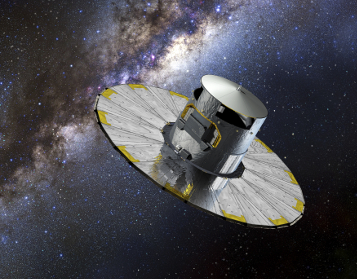
\includegraphics[width=1\linewidth]{GaiaIm}
    \caption{Gaia satellite}
  \end{subfigure}
     \begin{subfigure}[b]{0.2\linewidth}
    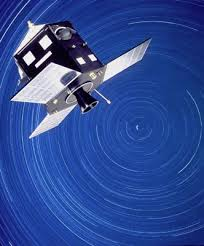
\includegraphics[width=1\linewidth]{hippSatIm}
     \caption{Hipparcos, the forerunner of Gaia}
  \end{subfigure}
\end{figure}

\end{itemize}
\end{frame}

\begin{frame}
\frametitle{The Goal of Our Research}
\begin{itemize}
\item Our goal is to extend galkin to gaia data
\item Galkin 12 contains 12 data sets analyzed by various collaborations
\item By consistently including more data, we can obtain a more accurate rotation curve
\begin{figure}[h!]
  \centering
  \begin{subfigure}[b]{0.4\linewidth}
    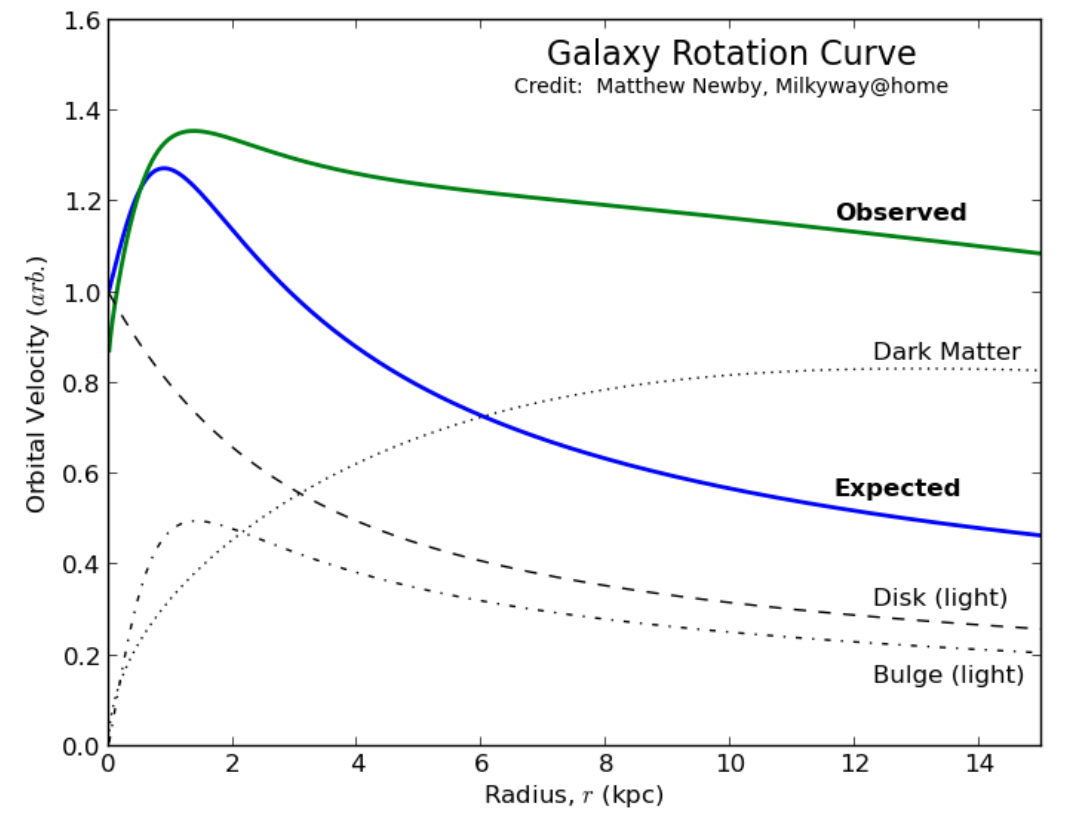
\includegraphics[width=\linewidth]{RotCurve}
  \end{subfigure}
    \caption{A typical rotation curve}
\end{figure}



\end{itemize}
\end{frame}

\begin{frame}
\frametitle{3 Baryonic Components of the Milky Way}
\begin{itemize}
\item The baryonic components of the Milky Way are:
\begin{itemize}
\item Bulge 
\item Thick disk  
\item Thin disk
\end{itemize}
\item Their corresponding densities are:
\begin{itemize}
\item  $\rho_{bulge}=\frac{\rho_{b,0}}{(1+r'/r_0)^\alpha} e^{[-(r'/r_{cut})^2]}$
\item $\rho_{disk}=\frac{\Sigma_{d,0}}{2 z_d} e^{(-\frac{|z|}{z_d}-\frac{R}{R_d})}$ (works for thin and thick disks)\\
\hspace*{\fill} \textcolor{blue} {McMillan, Arxiv:1102.4340}
\end{itemize}
\end{itemize}

\begin{figure}[h!]
  \centering
  \begin{subfigure}[b]{0.4\linewidth}
    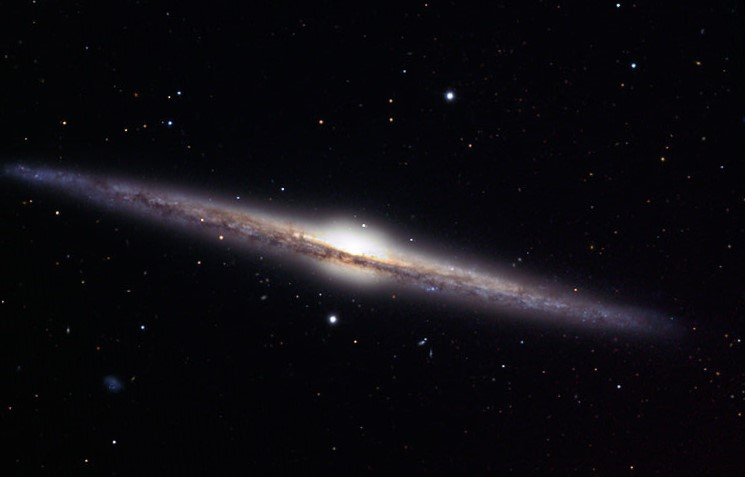
\includegraphics[width=\linewidth]{milkyWay}
  \end{subfigure}
    \caption{The Milky Way}
\end{figure}
\end{frame}

\begin{frame}
\frametitle{Circular Velocity of a Particle}
\begin{itemize}
\item Assume the only force is gravitational
\item $F=-\nabla U=-m \nabla \phi=m {v_c}^2/r \implies v_c=\sqrt{-r \nabla \phi}$
\item Where $\phi=-G \int \frac{\rho}{\scripty{r}} \mathrm{d} V$ is the gravitational potential

\end{itemize}
\end{frame}

\begin{frame}
\frametitle{Theoretical Rotation Curve (Baryons only)}
\begin{itemize}
\item Using $\rho=\rho_{bulge}+\rho_{thin\, disk}+\rho_{thick\, disk}$ to calculate Vc

\begin{figure}[h!]
  \centering
  \begin{subfigure}[b]{0.65\linewidth}
    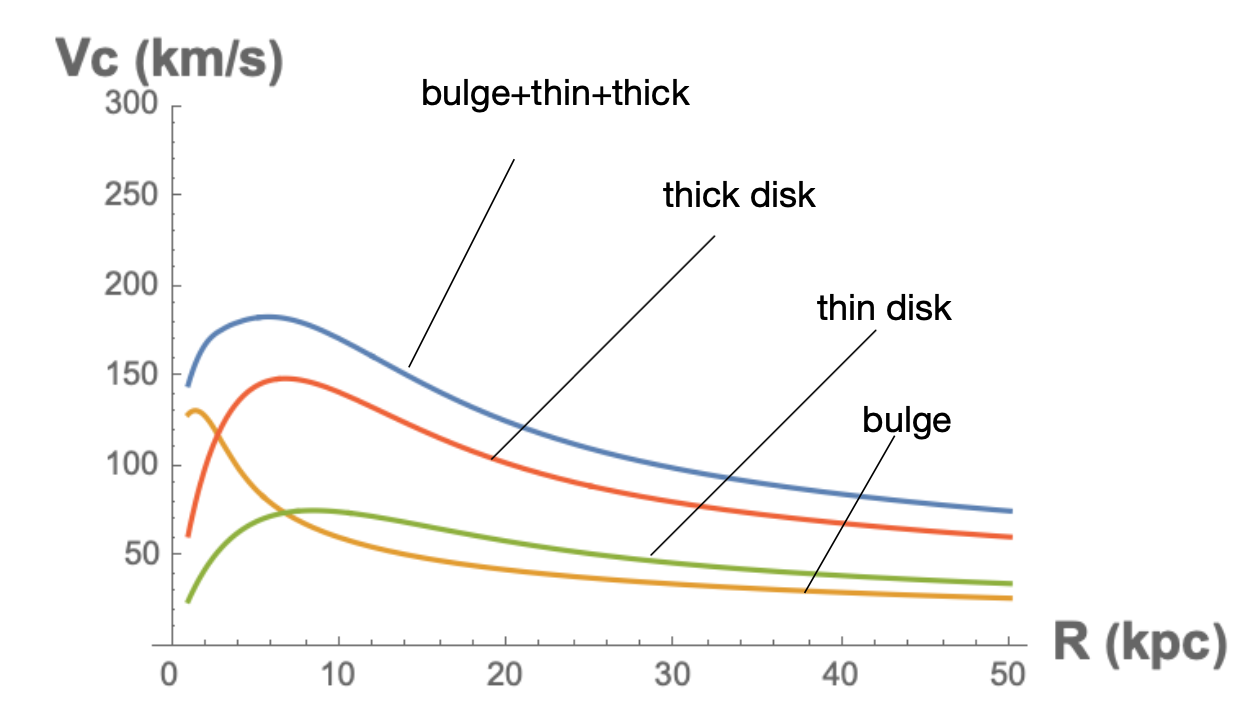
\includegraphics[width=\linewidth]{RotCurvTh252}
  \end{subfigure}
    \caption{Theoretical rotation curves from experimentally motivated models}
\end{figure}

\item $v_c(R)$ is called the rotation curve
\item So far we've considered only baryonic components
\item Alternatively, we can find $v_c(R)$ directly from the Gaia data

\end{itemize}
\end{frame}

\begin{frame}
\frametitle{First the Method}
\begin{itemize}
\item First we obtain the position of each star and transform to galactic coordinates (r,b,l)
\begin{itemize}
\item r is the distance to the star relative to the sun
\item r=1/p where p is the parallax
\item b is the galactic latitude of the star
\item l is the galactic longitude of the star
\item It will be useful to use a cartesian basis:
\item $\hat{x}$ points towards galactic center, $\hat{y}$ points towards increasing $l$, $\hat{z}$ points towards galactic north
\end{itemize}

\begin{figure}[h!]
  \centering
  \begin{subfigure}[b]{0.55\linewidth}
    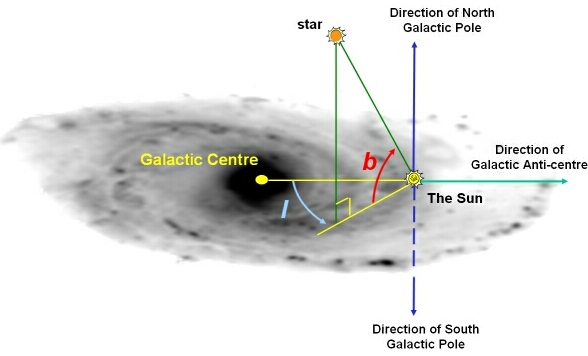
\includegraphics[width=\linewidth]{galCoordIm2}
  \end{subfigure}
    \caption{Galactic coordinate system}
\end{figure}


\end{itemize}
\end{frame}

\begin{frame}
\frametitle{First the Method}
\begin{itemize}
\item First, we calculate the position $\vec{r}_{sh}=(r \cos b \cos l,\, r \cos b \sin l, r \sin b)$
\item The velocity is $\vec{v}_{sh}=(-r(\mu_b \cos l \sin b + \mu_{l*} \sin l) + v_r \cos b \cos l,
r(-\mu_b \sin b \sin l + \mu_{l*} \cos l) + v_r \cos b \sin l, r \mu_b \cos b + v_r \sin b)$
\item Where $\mu_b=\dot{b}, v_r=\dot{r}, \mu_{l*}=\dot{l} \cos b$
\item Gaia DR2 contains quantities: $p, l, b, \mu_b, \mu_{l*}, v_r$
\item This gives us the velocity of the star (s) relative to the sun (h)
\item We need the velocity relative to the galactic center (c)
\item Using a Galilean transformation (vector addition) we obtain
\item $\vec{r}_{sc}=\vec{r}_{hc}+\vec{r}_{sh} \implies \vec{v}_{sc}=\vec{v}_{hc}+\vec{v}_{sh}$
\begin{itemize}
\item Where $\vec{r}_{hc}=(8.33,0,0.025)(kpc)$ and $\vec{v}_{hc}=( 11.10,  242.24,  7.25)(km/s)$
\hspace*{\fill} \textcolor{blue} {McMillan, Arxiv:1102.4340}
\end{itemize}


\end{itemize}
\end{frame}


\begin{frame}
\frametitle{Finding the Rotation Curve Obtained by Gaia}
\begin{itemize}
\item Like before, we care about stars that are close to the galactic plane and stars traveling in a circle
\item These stars have small radial velocities 
\item Lets also require the height is less than 100 pc of the galactic plane
\item Lets choose stars whose velocity is sufficiently tangential by requiring 
$|\frac{\vec{v}_{sc} \cdot \hat{r}_{sc}}{|\vec{v}_{sc}|}|< \epsilon$

\begin{figure}[h!]
  \centering
  \begin{subfigure}[b]{0.5\linewidth}
    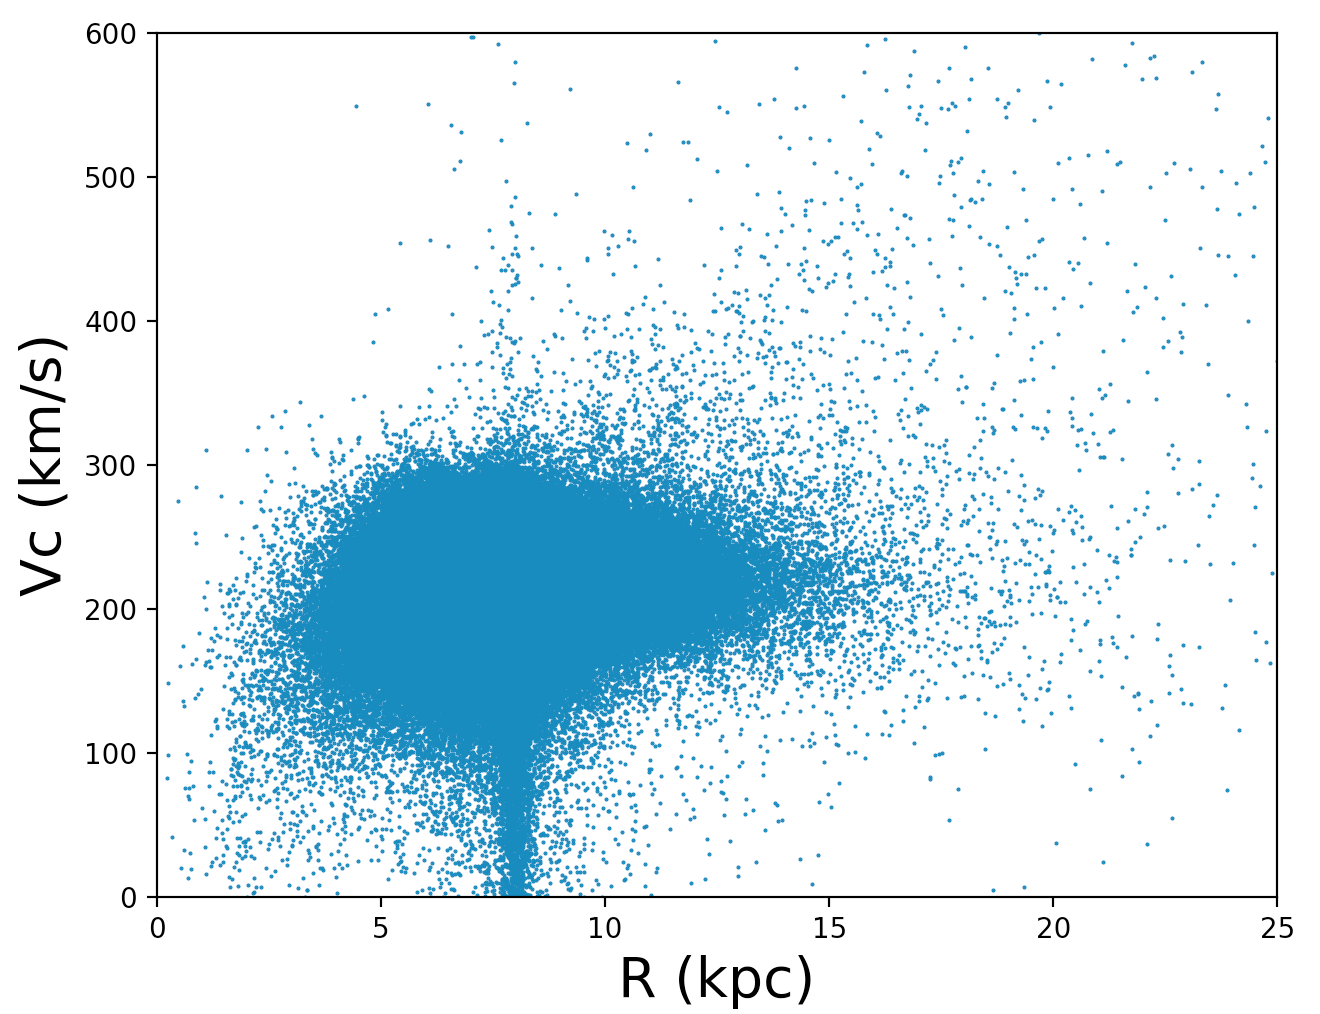
\includegraphics[width=\linewidth]{rotCurvBefBin3}
  \end{subfigure}
    \caption{$v_c$ vs. $R$ unbinned}
\end{figure}

\end{itemize}
\end{frame}


\begin{frame}
\frametitle{Actual Rotation Curve}
\begin{itemize}
\item After binning using a width of 0.5 kpc we obtain a preliminary rotation curve

%\begin{figure}[h!]
%  \centering
%  \begin{subfigure}[b]{0.4\linewidth}
%    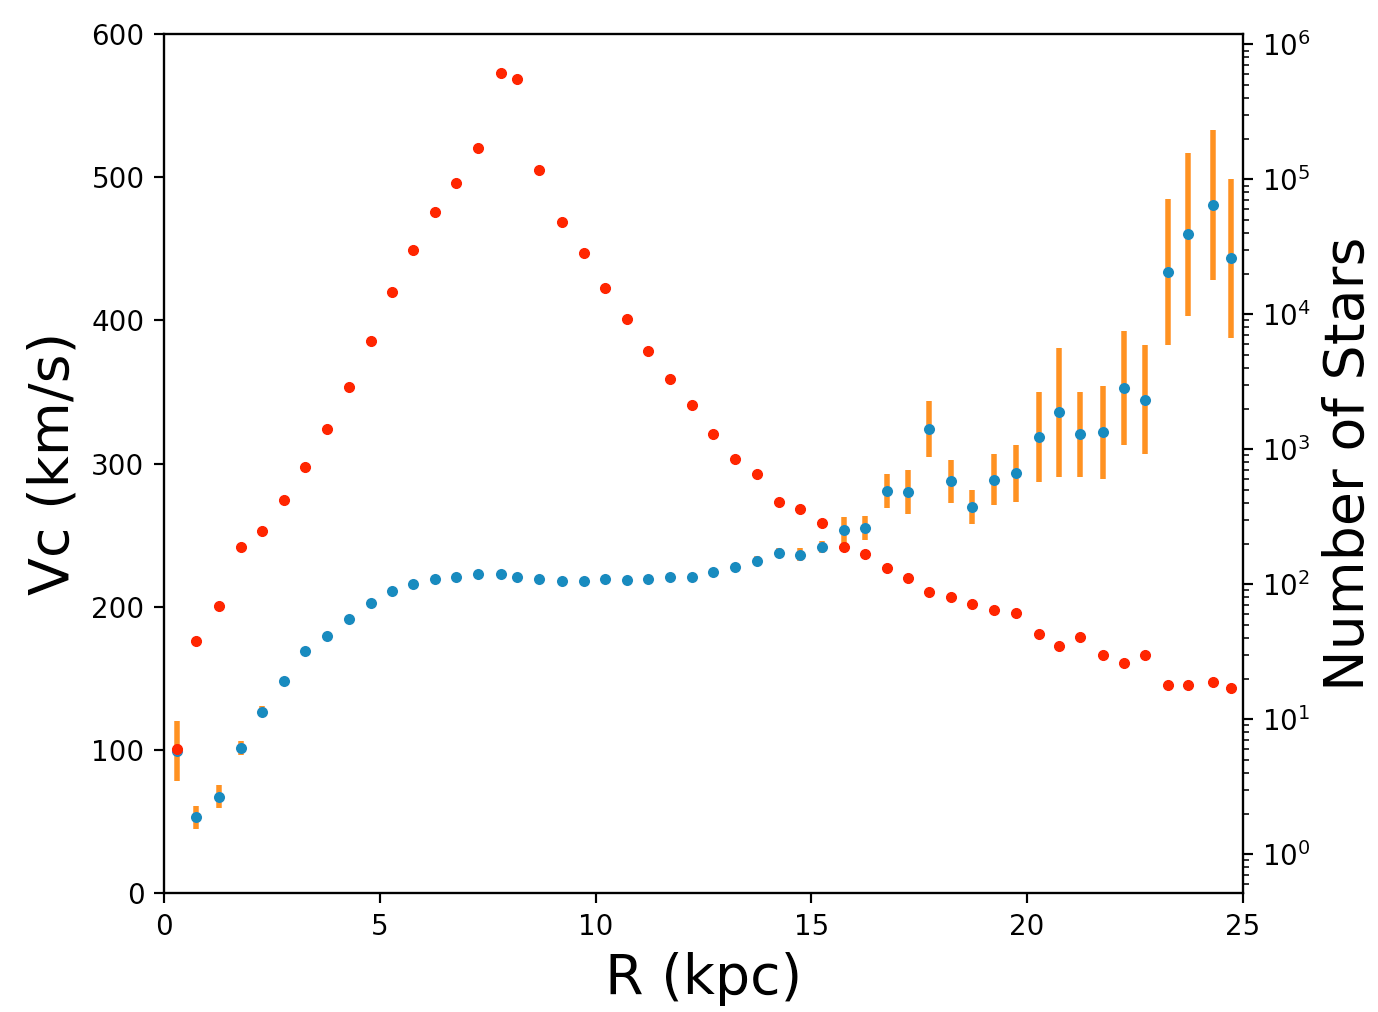
\includegraphics[width=1\linewidth]{rotCurvAftBin2}
%    \caption{Actual curve obtained from Gaia (errors are bootstrapped)}
%  \end{subfigure}
%     \begin{subfigure}[b]{0.55\linewidth}
%    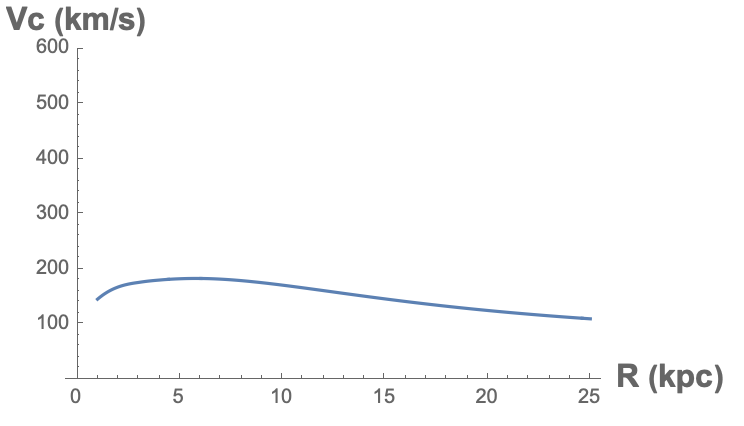
\includegraphics[width=1\linewidth]{RotCurvTh253}
%     \caption{Theoretical rotation curve found using observable mass density}
%  \end{subfigure}
%\end{figure}
\begin{figure}[h!]
  \centering
  \begin{subfigure}[b]{0.6\linewidth}
    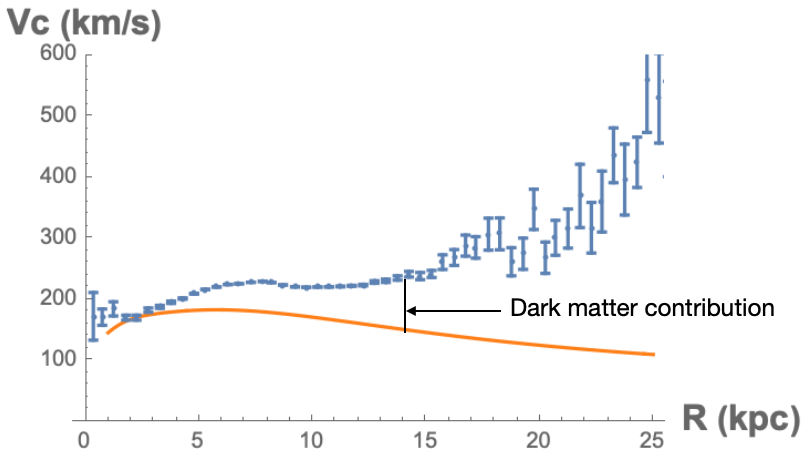
\includegraphics[width=\linewidth]{RotCurvAftBin3}
  \end{subfigure}
    \caption{Actual curve obtained from Gaia (blue) (errors are bootstrapped), Baryonic component (orange)}
\end{figure}

\item Next steps:
\begin{itemize}

\item Understand the sharp increase in velocity for large radii
\item Study matter morphology
\item Combine results with galkin
 \end{itemize}


\end{itemize}
\end{frame}




%------------------------------------------------



%----------------------------------------------------------------------------------------

\end{document} 